
\chapter{Evaluation}
\label{chap:evaluation}

This chapter addresses implementation details, experiments, ablation studies and achieved results.



\section{Training and validation data}

Each training session consists of optimizing parameters of a separate neural representation from one of proposed methods.
The dataset for each training session is created on one specific scene and with one specific light setting.
All of used datasets have been created in an artificial environment using Blender \cite{blender}.
Each dataset consists of rendered RGB images of the scene.
Each image is an HDR image (the OpenEXR \cite{openexr} format is used to store HDR data on disk).
The dataset samples are the aforementioned images
that correspond to a view from a pin-hole camera with intrinsic parameters $\mathcal{I}$ (same for the whole dataset).
The camera is placed on a sphere around the scene,
up-vector is always positive in $Z$ axis,
the orientation is always aimed to the center of the scene.
The position of the camera is described with two angles: azimuthal angle $\theta$ and inclination angle $\phi$.
For each view the values of $(\theta, \phi)$ are sampled uniformly on the surface of the sphere.
In the experiments the inclination angle is bounded between $-10$ and $80$ degrees.
Camera extrinsics (in form of transformation matrix) are exported for each dataset sample along with the HDR image.
Additionally to that the bounding box is also exported as it is required to initialize the octree for the NSVF method.


\subsection{Light settings}

Different light settings are required due to a diversity of tasks that different methods are to solve.
The illumination of the scene is set using point light source.
The intensity of the light source varies for different scenes and is chosen empirically.
The positioning of the light source is performed according to the chosen light setting.
Three different light settings are used in order to create three versions of each dataset.
This is done based on the fact that different methods can only handle datasets with different settings:
\begin{enumerate}
    \item \textbf{Static setting}
    
    In this case the light source positioned at the same global location for all of the dataset samples.
    This allows to produce renders of the scene with static illumination.
    The motivation for this type of datasets comes from the limitation of the NSVF method
    as it does not imply dynamic illumination.
    Datasets with static setting are made for 'Vanilla NSVF' (\cite{liu2021neural})
    and can also be processed with 'Brute-force' (\Cref{sec:explicit_scheme})
    and both explicit and implicit schemes (\Cref{fig:implicit_scheme})
    with in-voxel approximation (\Cref{sec:invoxel}).
    
    \item \textbf{Colocated setting}
    
    This setting implies the light source to be co-located with the camera.
    In this case there is no displacement between camera and light source,
    which allows the NRF (\cite{bi2020neural}) approach to reuse the view volume transmittances
    in calculations as transmittances of the light rays.
    The 'Brute-force' scheme as well as both explicit and implicit schemes
    with in-voxel approximation are also able to be trained on this type of datasets.
    
    \item \textbf{Arbitrary setting}
    
    Datasets that have been created with this setting consist of renders
    where both camera and light positions are sampled uniformly on a sphere around the scene.
    The positioning of the light source follows the same scheme as for camera position.
    Another constraint is applied here that forces the angle
    between view and light rays to the center of the scene to be smaller
    than some value $\alpha_{max}$.
    In the experiments the value $\alpha_{max} = 120$ degrees has been used.
    
    This setting is focused on general case of the NRF approach
    and can be handled by proposed methods, such as: 'Brute force' scheme
    and both explicit and implicit schemes with in-voxel approximation.
\end{enumerate}




\begingroup
\setlength{\tabcolsep}{40pt} % Default value: 6pt
\begin{figure}
    \centering
    \begin{tabular}{ccc}
          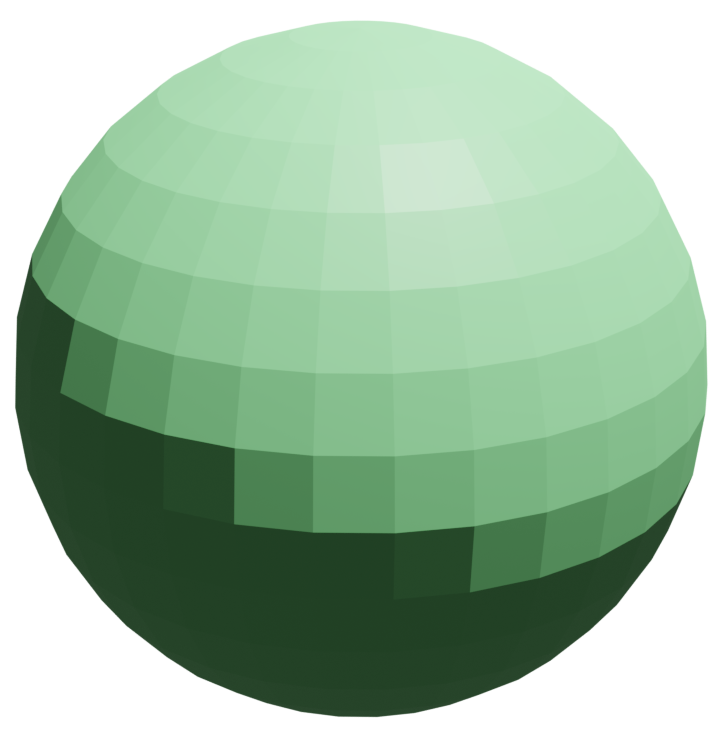
\includegraphics[width=0.13\textwidth]{figures/sphere.png}
          & 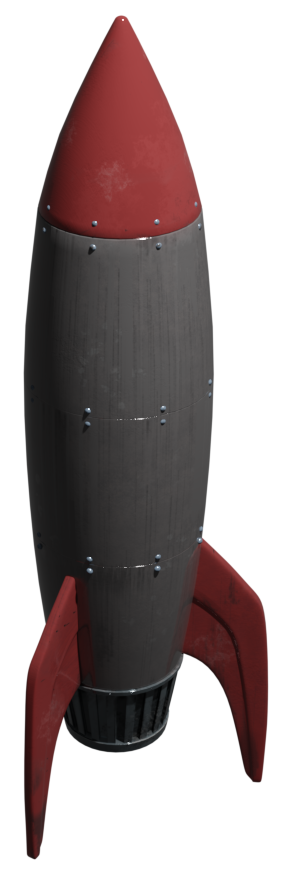
\includegraphics[width=0.1\textwidth]{figures/rocket.png}
          & 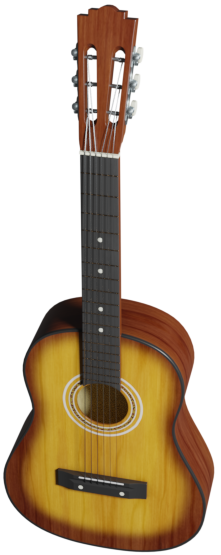
\includegraphics[width=0.13\textwidth]{figures/guitar.png}
          \\(a) Sphere & (b) Rocket & (c) Guitar
    \end{tabular}
    \caption{
    Preview samples of the created datasets.
    \im{how to align sphere in center?}
}
\label{fig:dataset_preview}
\end{figure}
\endgroup

\subsection{Scenes}

Creating the datasets from scratch is motivated by the fact that
vast majority of related works do not consider any light interaction.
This results in such a problem that the datasets that have been used in these works
do not include any necessary light information (global position).
Another limitation of these datasets is that the light source is static upon the dataset samples,
which results in a sparse light-view sampling of the scene.
Three different scenes have been used for the evaluation.
\im{reference figure to show this off - say about tonemapping}

\textbf{Sphere}

The \textit{sphere} scene consists solely of a sphere,
which shares Lambertian reflectance (\cite{blinn1982light}) with some specular and roughness components.
This scene is mostly used as a baseline as it is a very simple
both geometrically and in terms of appearance.

\textbf{Rocket}

The \textit{rocket} scene contains a single object,
which exhibits complicated geometry and realistic non-Lambertian materials.
This scene contains global geometry complications (rocket wings) and some fine details (rivets on the rocket shell).
The surface of the rocket shows moderate level of specularities (in comparison with sphere scene)

\textbf{Guitar}

The \textit{guitar} scene is created for testing models ability
to reproduce highly specular BRDFs.
Complex geometry also allows to asses how model handles geometrical features on different scales.
For example strings can be barely seen on renders and they would presumably the most troublesome geometrical part of the whole scene.



\subsection{Real-world dataset}

\im{About how to get camera positions}

\im{Description of faulty flower dataset??}


% \begin{enumerate}
%     \item Synthetic datasets:
%     \begin{enumerate}
%         \item static/co-located/arbitrary
%         \item Blender + python
%         \item Blender point light intensity for light attenuation
%         \item Different scenes (with its features explanations: reflectance, shape, etc.)
%     \end{enumerate}
%     \item Real-world datasets: flower??? tac7
% \end{enumerate}


\section{Implementation details}

\begin{enumerate}
    \item Loss function: color + beta-regularizer
    \item Parameters: optimizer, lr, batch, coefficients, pruning/refinement iterations
    \item Software/Hardware setup
    \item Time estimates
\end{enumerate}



\section{Metrics}

Metrics: MSE, SSIM, FLIPLoss/HDRFlipLoss


\section{Experiments}

The experiments involve training models on different synthetic datasets (\im{reference to prev. subsection}) with different parameters
and quantitative (\im{ref}) and qualitative (\im{ref}) comparisons of those.



\section{Comparisons}

Following models for comparison:
\begin{enumerate}
    \item Vanilla NSVF
    \item Explicit scheme colocated (NRF+NSVF)
    \item Explicit scheme 'brute-force'
    \item Explicit scheme w/in-voxel approximation
    \item Implicit scheme w/in-voxel approximation
\end{enumerate}


Following datasets for comparison:
\begin{enumerate}
    \item BRDF sphere
    \item Rocket
    \item Guitar
    \item \color{orange}{Trophy/donut/tablelamp}
\end{enumerate}

Following settings:
\begin{enumerate}
    \item Static
    \item Colocated
    \item Arbitrary
\end{enumerate}


Table with time/memory consumptions:

\im{I'M TABLE!}


\section{Discussion}

\begin{enumerate}
    \item HDR inputs: preprocessing (log-transform)
    \item Background color problem?
    \item In-Voxel approximation: different sigma strategies
    \item Implicit scheme with tangential coordinate system
\end{enumerate}


% \section{Colocated setting flaws}

% Network barely generalizes for noncolocated light source position when trained only on colocated setting


% \section{Brute Force vs Approximation}






% \section{Blender-Radiance coefficient}

% The light attenuation factor has to be taken into account in the explicit scheme.

% $L_o(x, \Omega_o) = L_e(x, \Omega_o) + \int_{H_i}{f_{BRDF}(\Omega_i, x, \Omega_o) L_i(x, \Omega_i) cos \Theta_i d\omega_i}$

% $L_i = \tau_l L_l$

% $L_l = f_{att}I$

% $f_{att}=\frac{1}{1 + 2d/r + d/r^2}$

% $L_o = \frac{k_d}{\pi} \frac{1}{1 + 2d/r + d/r^2} I cos \Theta_i$

% $k_c = 0, k_l = 0, k_q = 1$

% r = 0.05

% $f_{att} = r^2 / d = 0.0025 / (10-0.05) = 2.51256e-4$

% $0.24316406 = 0.8 / \pi * 2.51256e-4 * I * 1$

% $0.24316406 = 2.01005e-4 * I$

% $I = 500$





% This is some test area for new mathematical helper macros to nicely visualize mathematical formulas.

% \section{Numbers}
% \begin{align}
%     \mathbb{C}
%     \qquad
%     \mathbb{R}
%     \qquad
%     \mathbb{Q}
%     \qquad
%     \mathbb{Z}
%     \qquad
%     \mathbb{N}
% \end{align}

% \section{Numbers with physical units}
% \begin{align}
%     \SI{1.23}{\meter\per\second}
% \end{align}
% \begin{align}
%     \si{\meter\per\second}
% \end{align}
% \begin{align}
%     \SI{1.23\pm0.45}{\meter\per\second}
% \end{align}
% \begin{align}
%     \SI{3e8}{\meter\per\second}
% \end{align}
% \begin{align}
%     \SI{32}{\giga\byte} = \SI{32e9}{\byte}
% \end{align}
% \begin{align}
%     \SI{32}{\gibi\byte} = \SI[exponent-base=2]{32e30}{\byte}
% \end{align}

% \section{Norm, Dot, Abs, Interval}
% \begin{align}
%     \pi = \const
% \end{align}
% \begin{align}
%     1 \in \interval{0}{2}
% \end{align}
% \begin{align}
%     1 \in \order{n}
% \end{align}
% \begin{align}
%     \evalat{ \frac{\partial f}{\partial x} }{ x = 0 }
% \end{align}
% \begin{align}
%     \norm{p} \qquad \norm{\frac{p}{2}}
% \end{align}
% \begin{align}
%     \abs{p} \qquad \abs{\frac{p}{2}}
% \end{align}
% \begin{align}
%     \dotproduct{p}{q} \qquad \dotproduct{\frac{p}{2}}{q}
% \end{align}
% \begin{align}
%     \crossproduct{p}{q} \qquad \crossproduct{\frac{p}{2}}{q}
% \end{align}

% \section{Vector, Matrix}
% \begin{align}
%     \vec{p} \qquad \vecarrow{p}
% \end{align}
% \begin{align}
%     \vec{p}^{\transposed}
% \end{align}
% \begin{align}
%     \gradient{\vec{p}}
% \end{align}
% \begin{align}
%     \divergence{\mat{A}}
% \end{align}
% \begin{align}
%     \laplacian{\mat{A}}
% \end{align}
% \begin{align}
%     \mat{A}
% \end{align}
% \begin{align}
%     \set{K} , K
%     \qquad
%     \set{N} , N
% \end{align}
% \begin{align}
%     \neighborhood{\vec{p}} = \left\{ \vec{q} \mid \norm{\vec{p} - \vec{q}} < \epsilon \right\}
% \end{align}

% \section{Set operations}
% \begin{align}
%     A \intersect B
% \end{align}
% \begin{align}
%     A \union B
% \end{align}
% \begin{align}
%     A \difference B
% \end{align}

% \section{Derivative, Integral, Sum, Probability}
% \begin{align}
%     \int_H x \, dx
% \end{align}
% \begin{align}
%     \sum_H x
% \end{align}
% \begin{align}
%     \probability{x}
% \end{align}
% \begin{align}
%     \probabilitygiven{x}{y}
% \end{align}
% \begin{align}
%     \expectation{x}
% \end{align}
% \begin{align}
%     \deviation{x}
% \end{align}
% \begin{align}
%     \variance{x}
% \end{align}


% \section{Lemma, Theorem, Corollary}
% \begin{lemma}
%     This is a lemma.
% \end{lemma}
% \begin{proof}
%     Proof of lemma.
% \end{proof}

% \begin{theorem}
%     This is a theorem.
% \end{theorem}
% \begin{proof}
%     Proof of theorem.
% \end{proof}

% \begin{corollary}
%     This is a corollary.
% \end{corollary}
% \begin{proof}
%     Proof of corollary.
% \end{proof}